%\title{Using the forest package to create trees in LaTeX}
% From http://tex.stackexchange.com/a/108728/23931 
\documentclass[12pt,preview,border=0]{standalone}
\usepackage[paperheight=8cm,paperwidth=7.5cm]{geometry}
\usepackage{graphicx}
% \usepackage{forest}
\usepackage{amsmath}
% \usepackage{txfonts}  %pretty math font
\usepackage{kmath,kerkis}
\usepackage{tikz}
\usetikzlibrary{arrows,automata,positioning}


%         R <--- Ow
%        ^ ^     /
%       /   \   /
%      /     \ v
%     J       W

\begin{document} 
\begin{center}
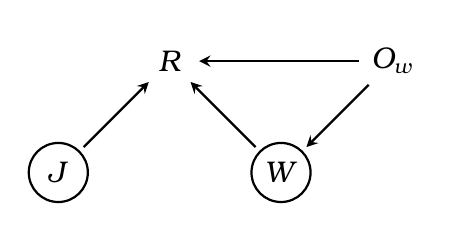
\begin{tikzpicture}[
	> = stealth, % arrow head style
	% shorten > = 1pt, % don't touch arrow head to node
	auto,
	node distance = 2cm, % distance between nodes
	thick, % line style
	U/.style={circle, draw=black, inner sep=0pt, outer sep=2.3pt, minimum size=7.5mm, font=\large},  %draw=black, fill=white
	O/.style={circle, inner sep=2.3pt, outer sep=0pt, minimum size=7.5mm, font=\large},              %draw=white, fill=white
	]
	
	% Nodes and their relative positions
	% t = 0
    \node[U] (W) {$W$};
    \node[O] (R)  [above  left of = W] {$R$};
    \node[O] (Ow) [above right of = W] {$O_w$};
    \node[U] (J) [below left of = R] {$J$};	
    
       
	% Paths connecting nodes
    \path[->] (J) edge (R);
    \path[->] (W) edge (R);
    \path[->] (Ow) edge (R);
    \path[->] (Ow) edge (W);
\end{tikzpicture}
	
\end{center}\end{document}
